%
\section{Introduction}
\label{sec:intro}


\cxj{Is your goal reconstruction or building extraction? The introduction should explain the overall goal. What are the challenges for building modeling from remote sensing images? What kind of work has been done in the literature? Why do we focus on building detection? What are our contributions?}

\IEEEPARstart{B}{uilding} extraction, which aims to extract rooftop in a large-scale remote sensing image, remains one of the main challenges in the field of remote sensing for several decades. In addition, automatic extraction of building rooftops from aerial and satellite imagery is an important step in many applications, such as: urban planing, automated map making, 3D city modeling, updating geographical dataset and military reconnaissance. It is particularly difficult to extract rooftop from remote sensing images at the pixel level because of the following three reasons: \romannumeral1) Density of the structures in the scene. A rural scene has low density but an urban scene has high density, with a suburban scene in between (medium density).  \romannumeral2) Shape of the structure. Buildings come in many shapes from simple rectangular blocks with flat roof to complex shapes with intricate, multi-based roof structure.  \romannumeral3) Image quality. Images vary in terms of contrast, resolution, and visibility  \cite{IEEEexample:huertas1988detecting}. Some remote sensing patches are shown in Fig.~\ref{fig:intro} \cxj{do not use the figure no directly. using ref{}..} , which illustrate the difficulties of building extraction task. 


\begin{figure}
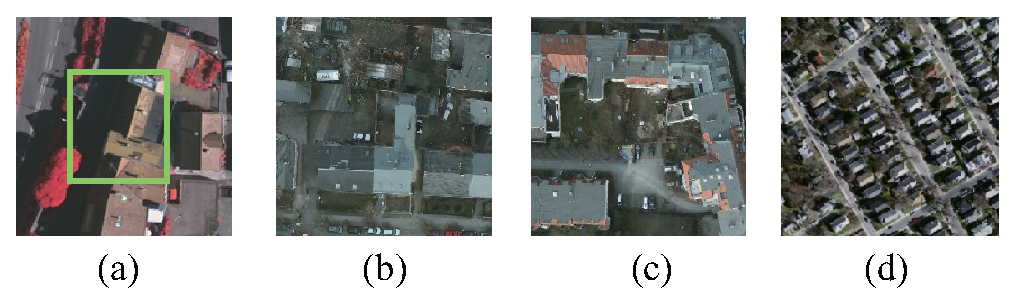
\includegraphics[width=8.7cm]{Figures/challenge.eps}
\caption{Examples of remote sensing patches with different kinds of challenges. (a) Shadow occlusion in green frame. (b) Low inter-class differences. (c) High intra class variance. (d) A lot of tiny buildings close to each other.}
\label{fig:intro}
\end{figure}


In the past decades, many researchers made some experimental investigations to extract buildings automatically. In the early days, many knowledge-based methods were put forward by \cite{IEEEexample:huertas1988detecting}, \cite{IEEEexample:noronha2001detection}, \cite{IEEEexample:nosrati2009novel}, \cite{IEEEexample:izadi2012three}, \cite{IEEEexample:wang2015efficient} whose basic ideas are derived from prior knowledge of buildings, for instance, buildings are closed polygons made up of some straight lines. Some others are energy based methods which mainly includes the variational level set evolution, improved snake model and graph cut \cite{IEEEexample:cote2013automatic}, \cite{IEEEexample:peng2005improved}, \cite{IEEEexample:sirmacek2009urban}.


In recent years, with the development of machine learning, many machine-learning techniques are gradually penetrating into the remote sensing domain. 
At first, some shallow networks were proposed for multiple object extraction\cite{IEEEexample:mnih2013machine}, \cite{IEEEexample:saito2016multiple}, \cite{IEEEexample:alshehhi2017simultaneous},\cite{IEEEexample:zhao2017contextually}. Afterwards, with increasing computer power, deep learning developed rapidly and introduced into the field of remote sensing. At the same time, some researchers tried Convolutional Neural Networks (CNNs) for aerial images classification and semantic pixel labelling~\cite{IEEEexample:paisitkriangkrai2015effective}, \cite{IEEEexample:liu2017dense}, \cite{IEEEexample:audebert2017deep}, \cite{IEEEexample:kampffmeyer2017urban}, \cite{IEEEexample:he2017multi}.


In this work, we propose a modified CNN architecture to extract buildings from satellite imagery. In our network, we want to take full advantages of the low-level appearance information as well as high-level semantic information. 
Therefore, we use not only the final prediction result obtained by CNN, but also the feature maps of other layers. Numerous experiments are conducted on three remote sensing image datasets and all obtain fairly good results. After rooftop extracting, the depth map is used to create the point cloud of rooftop. Based on the point cloud, the 3D models are carried out using the method proposed by Zhou\cite{IEEEexample:zhou20112}. Fig.~\ref{fig:overview} illustrates pipeline of our work. Our technical contributions are: 
%
\begin{enumerate}
	\item A novel HF-FCN which is specially designed for multi-scale building extraction is proposed. It can deal with the problems of different sizes, diverse appearance and mutual occlusion of buildings and etc. The overall accuracy based on HF-FCN exceeds the state-of-art algorithms.
	\item Our approach are significantly computationally efficient than existing techniques.
	\item A complete system for building extraction and 3D modelling of large-scale urban areas is proposed. And the building extraction part is a end-to-end network that does not need any post processing.
\end{enumerate}
 
\begin{center}
\begin{figure}
\includegraphics[width=8.7cm]{Figures/pipeline.eps}
\caption{An overview of proposed urban 3D modelling framework. The inputs of our system are multi-channel images. Semantic segmentation that extracts building areas from aerial images is the first step. After it, we generate the point cloud according to the DSM. Based on the point cloud, the 3D reconstruction is implemented.}
\label{fig:overview}
\end{figure}
\end{center} 



The remainder of this paper is organized as follows. Sec.~\ref{Sec:RelatedWork} sums up the related past works. In Sec.~\ref{Sec:HF-FCN}, we introduce the architecture of our network and show the training steps. And in Sec.~\ref{Sec:exp}, a brief description of the dataset used for our task is provided. HF-FCN training strategies, details and its evaluation metrics are also described. In Sec.~\ref{Sec:Res} we present the experimental and 3D modelling results. 
Finally, the conclusion and discussion are discussed in Sec.~\ref{Sec:Con}.
